\chapter{ESRGAN}

Kolejny omawiany algorytm rozwiązuje problem super-rozdzielczości obrazów przy użyciu Generatywnych Sieci Przestawnych. Algorytm został opracowany przez: Xintao Wang, Ke Yu, Shixiang Wu, Jinjin Gu, Yihao Liu,
Chao Dong, Chen Change Loy, Yu Qiao, Xiaoou Tang \cite{wang2018esrgan}.




\begin{figure}[ht]
    \centering
    \begin{minipage}[t]{0.4\linewidth}
        
\includegraphics[width=\linewidth]{Rozdziały/02.Podstawy_teoretyczne/Obrazy/comic.png}
        \caption{Obraz wejściowy}
        \label{fig:image60}
    \end{minipage}
    \hspace{0.5cm}
    \begin{minipage}[t]{0.4\linewidth}
        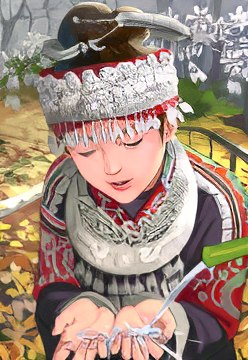
\includegraphics[width=\linewidth]{Rozdziały/02.Podstawy_teoretyczne/Obrazy/comic_ESRGAN_x4.png}
        \caption{Obraz powiększony algorytmem \textbf{ESRGAN} czterokrotnie}
        \label{fig:image61}
    \end{minipage}
\end{figure}


\section{Architektura ESRGAN}


Szczegółowy opis architektury sieci ESRGAN, w tym jej głównych komponentów i zasady działania.



% \section{Kluczowe cechy i innowacje}


Omówienie innowacji wprowadzonych w ESRGAN i w jaki sposób różnią się one od wcześniejszych podejść.



\section{Proces treningu i implementacji}


Opis procesu treningu sieci ESRGAN, w tym zbierania danych, uczenia oraz wyzwań implementacyjnych.



\section{Przykłady zastosowań i rezultaty}


Prezentacja przykładów, gdzie ESRGAN został użyty oraz analiza wyników, jakie osiągnięto dzięki tej technologii.